\ESKDappendix{обязательное}{Описание экспериментов по проверке состоятельности использованных методов локализации робота с помощью сторонней системы технического зрения}\label{app_cv_system}

Система технического зрения (СТЗ) представляет собой веб-камеру Logitech C920 FullHD закрепленную над зоной проведения экспериментов на высоте $2.85$ метра. Камера подключена к стационарному компьютеру, не связанному с роботом, на котором запускается программа на языке программирования Python. Для решения задач СТЗ используется библиотека OpenCV. На роботе закреплена плоская панель с двумя маркерами: синим -- над задней осью и красным -- в передней части робота. Центр масс синего маркера располагается над точкой $C$ (см. рисунок~\ref{img_kinematic_model_picture}).

СТЗ работает по следующему алгоритму:
\begin{enumerate}
	\item каждый из кадров видео-потока представляется в цветовом пространстве HSV (Hue, Saturation, Value);
	\item из кадра выделяются области с красным и синим цветам;
	\item вычисляются координаты маркеров в СК кадра в пикселях;
	\item координаты переводятся из пикселей в метры в соответствии со следующим выражением:
	\begin{equation}
		d_{m} = d_{px} \cfrac{D_{m}}{D_{px}}
	\end{equation}
	где $d_{m}$ и $d_{px}$~--- координата или размер объекта в метрах и пикселях, соответственно; $D_{m}$ и $D_{px}$~--- длина диагонали кадра в метрах и пикселях;
	\item то место, где стоит робот при запуске СТЗ, принимается за базовую СК (она же является базовой и для одометрии);
	\item по расположению красного маркера относительно синего рассчитывается ориентация робота;
	\item все последующие координаты робота и его ориентации выражаются в базовой СК;
	\item значения координат и ориентация робота записываются в файл и выводятся на кадре.  
\end{enumerate}

Для проверка СТЗ был проведен эксперимент:
\begin{enumerate}
	\item при помощи отвеса и двух человек, камера была установлена так, чтобы оптическая ось была строго перпендикулярна плоскости пола зоны эксперимента;
	\item на полу были отмечены четыре точки и измерены расстояния между ними;
	\item последовательно в каждую точку ставился робот так, чтобы точка $C$ (или что то же самое -- центр масс синего маркера) была над отмеченной на полу точкой;
	\item фиксировался результат в виде скриншота с отмеченными на нем координатами робота. 
\end{enumerate}

Результаты работы СТЗ при проверке приведены на рисунке~\ref{cv_check}. Результаты проверки приведены в таблице~\ref{cv_check_results}.

Смотря на результаты проверки разработанной в этой работе СТЗ можно заключить о невозможности достоверного определения траектории движения робота. Так как во-первых, изображение получаемое с камеры имеет дисторсию, что наглядно видно на рисунке~\ref{map_real} (растянутая в нижней части кадра рулетка имеет видимый изгиб), а также из таблицы~\ref{cv_check_results} (расстояния между точкой в центре кадра и близкими к нему точками имеют меньшую ошибку, чем расстояние до точки у края) и, во-вторых, проверка СТЗ проводилась <<на скорую руку>>, в связи с чем были допущены, возможно, существенные ошибки при экспериментах.

\begin{figure}[h!]
	\begin{minipage}[h]{0.47\textwidth}
		\centering{ 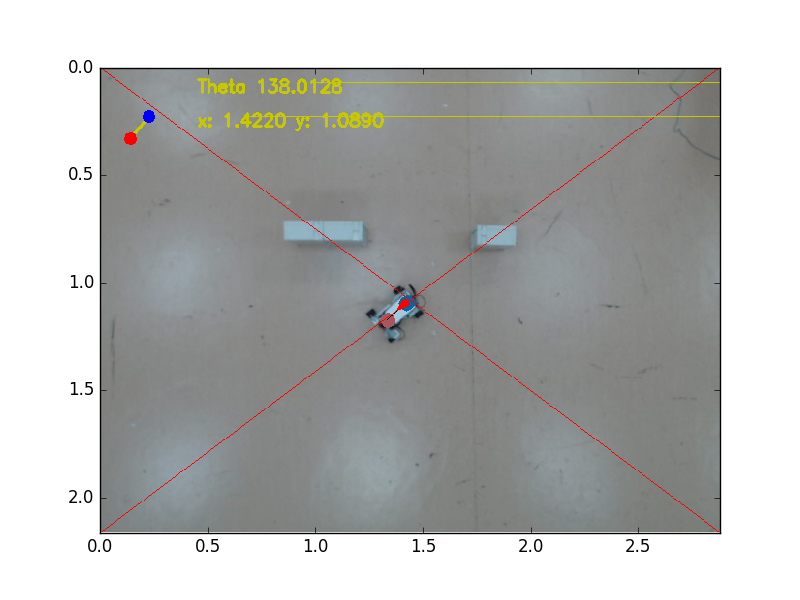
\includegraphics[width=\textwidth]{img/cv_2.png} \\ a) (1.422, 1.089)}
	\end{minipage}
	\hfill
	\begin{minipage}[h]{0.47\textwidth}
		\centering{ 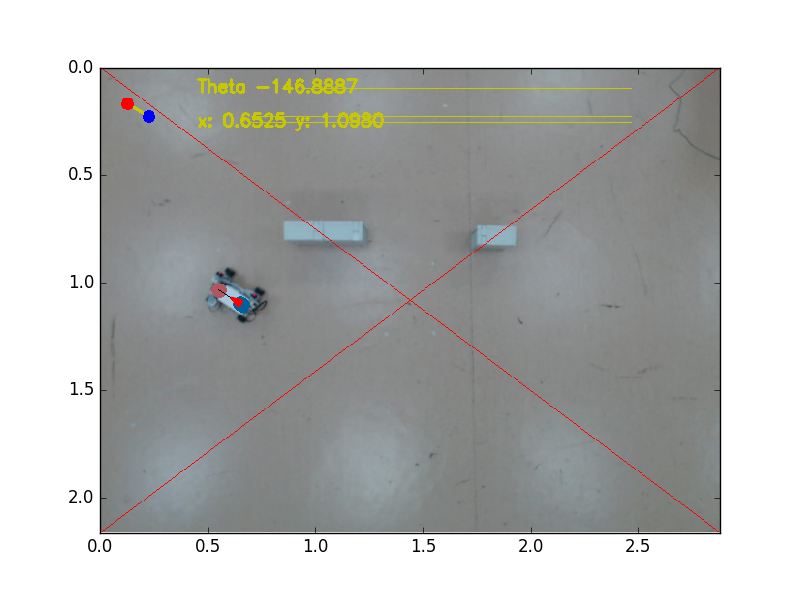
\includegraphics[width=\textwidth]{img/cv_3.png} \\ б) (0.6525, 1.098)}
	\end{minipage}
	\vfill
	\begin{minipage}[h]{0.47\textwidth}
		\centering{ 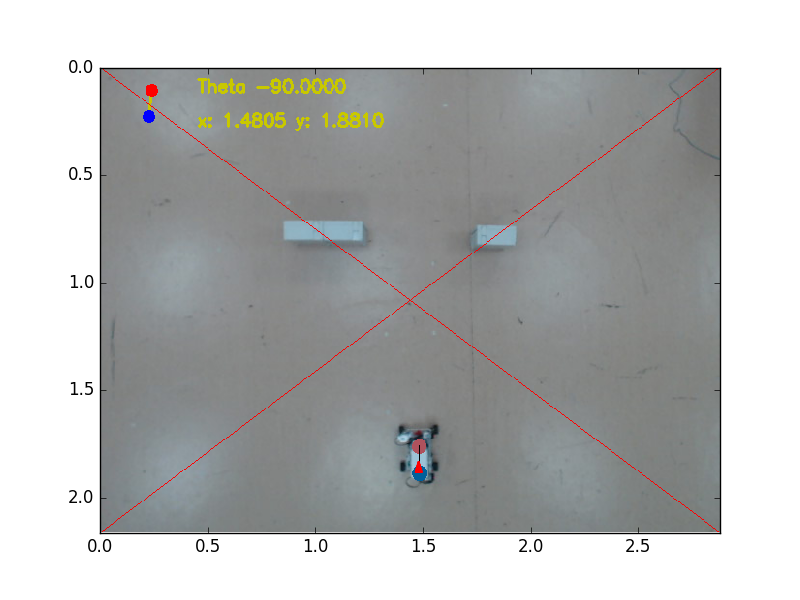
\includegraphics[width=\textwidth]{img/cv_1.png} \\ в) (1.4805, 1.881)}
	\end{minipage}
	\hfill
	\begin{minipage}[h]{0.47\textwidth}
		\centering{ 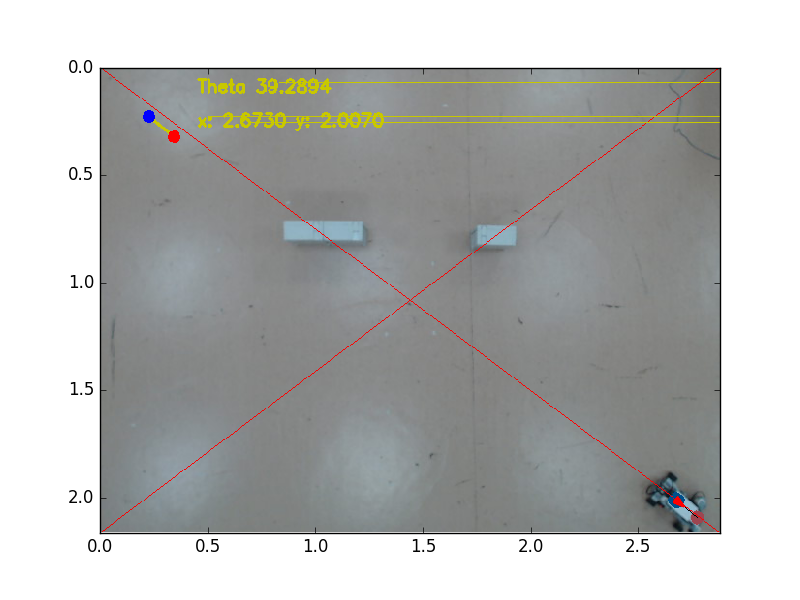
\includegraphics[width=\textwidth]{img/cv_4.png} \\ г) (2.673, 2.007)}
	\end{minipage}
	\caption{Проверка СТЗ.}
	\label{cv_check}
\end{figure}

\begin{table}[h!]
	\centering
	\caption{Результаты проверки СТЗ}
	\label{cv_check_results}
	\begin{tabular}{llll}
		\multicolumn{1}{c}{\begin{tabular}[c]{@{}c@{}}Расстояние \\ между точками\end{tabular}} & СТЗ, м & Линейка, м & Ошибка, м \\
		а и б & 0.7695 & 0,75 & 0.0194 \\
		а и в & 0.7941 & 0,75 & 0.0441 \\
		а и г & 1.5516 & 1,44 & 0.1116
	\end{tabular}
\end{table}

\clearpage
Сравнение траекторий с СТЗ и одометрии приведено на рисунке~\ref{cv_trajectory}
\begin{figure}[h]
	\centering
	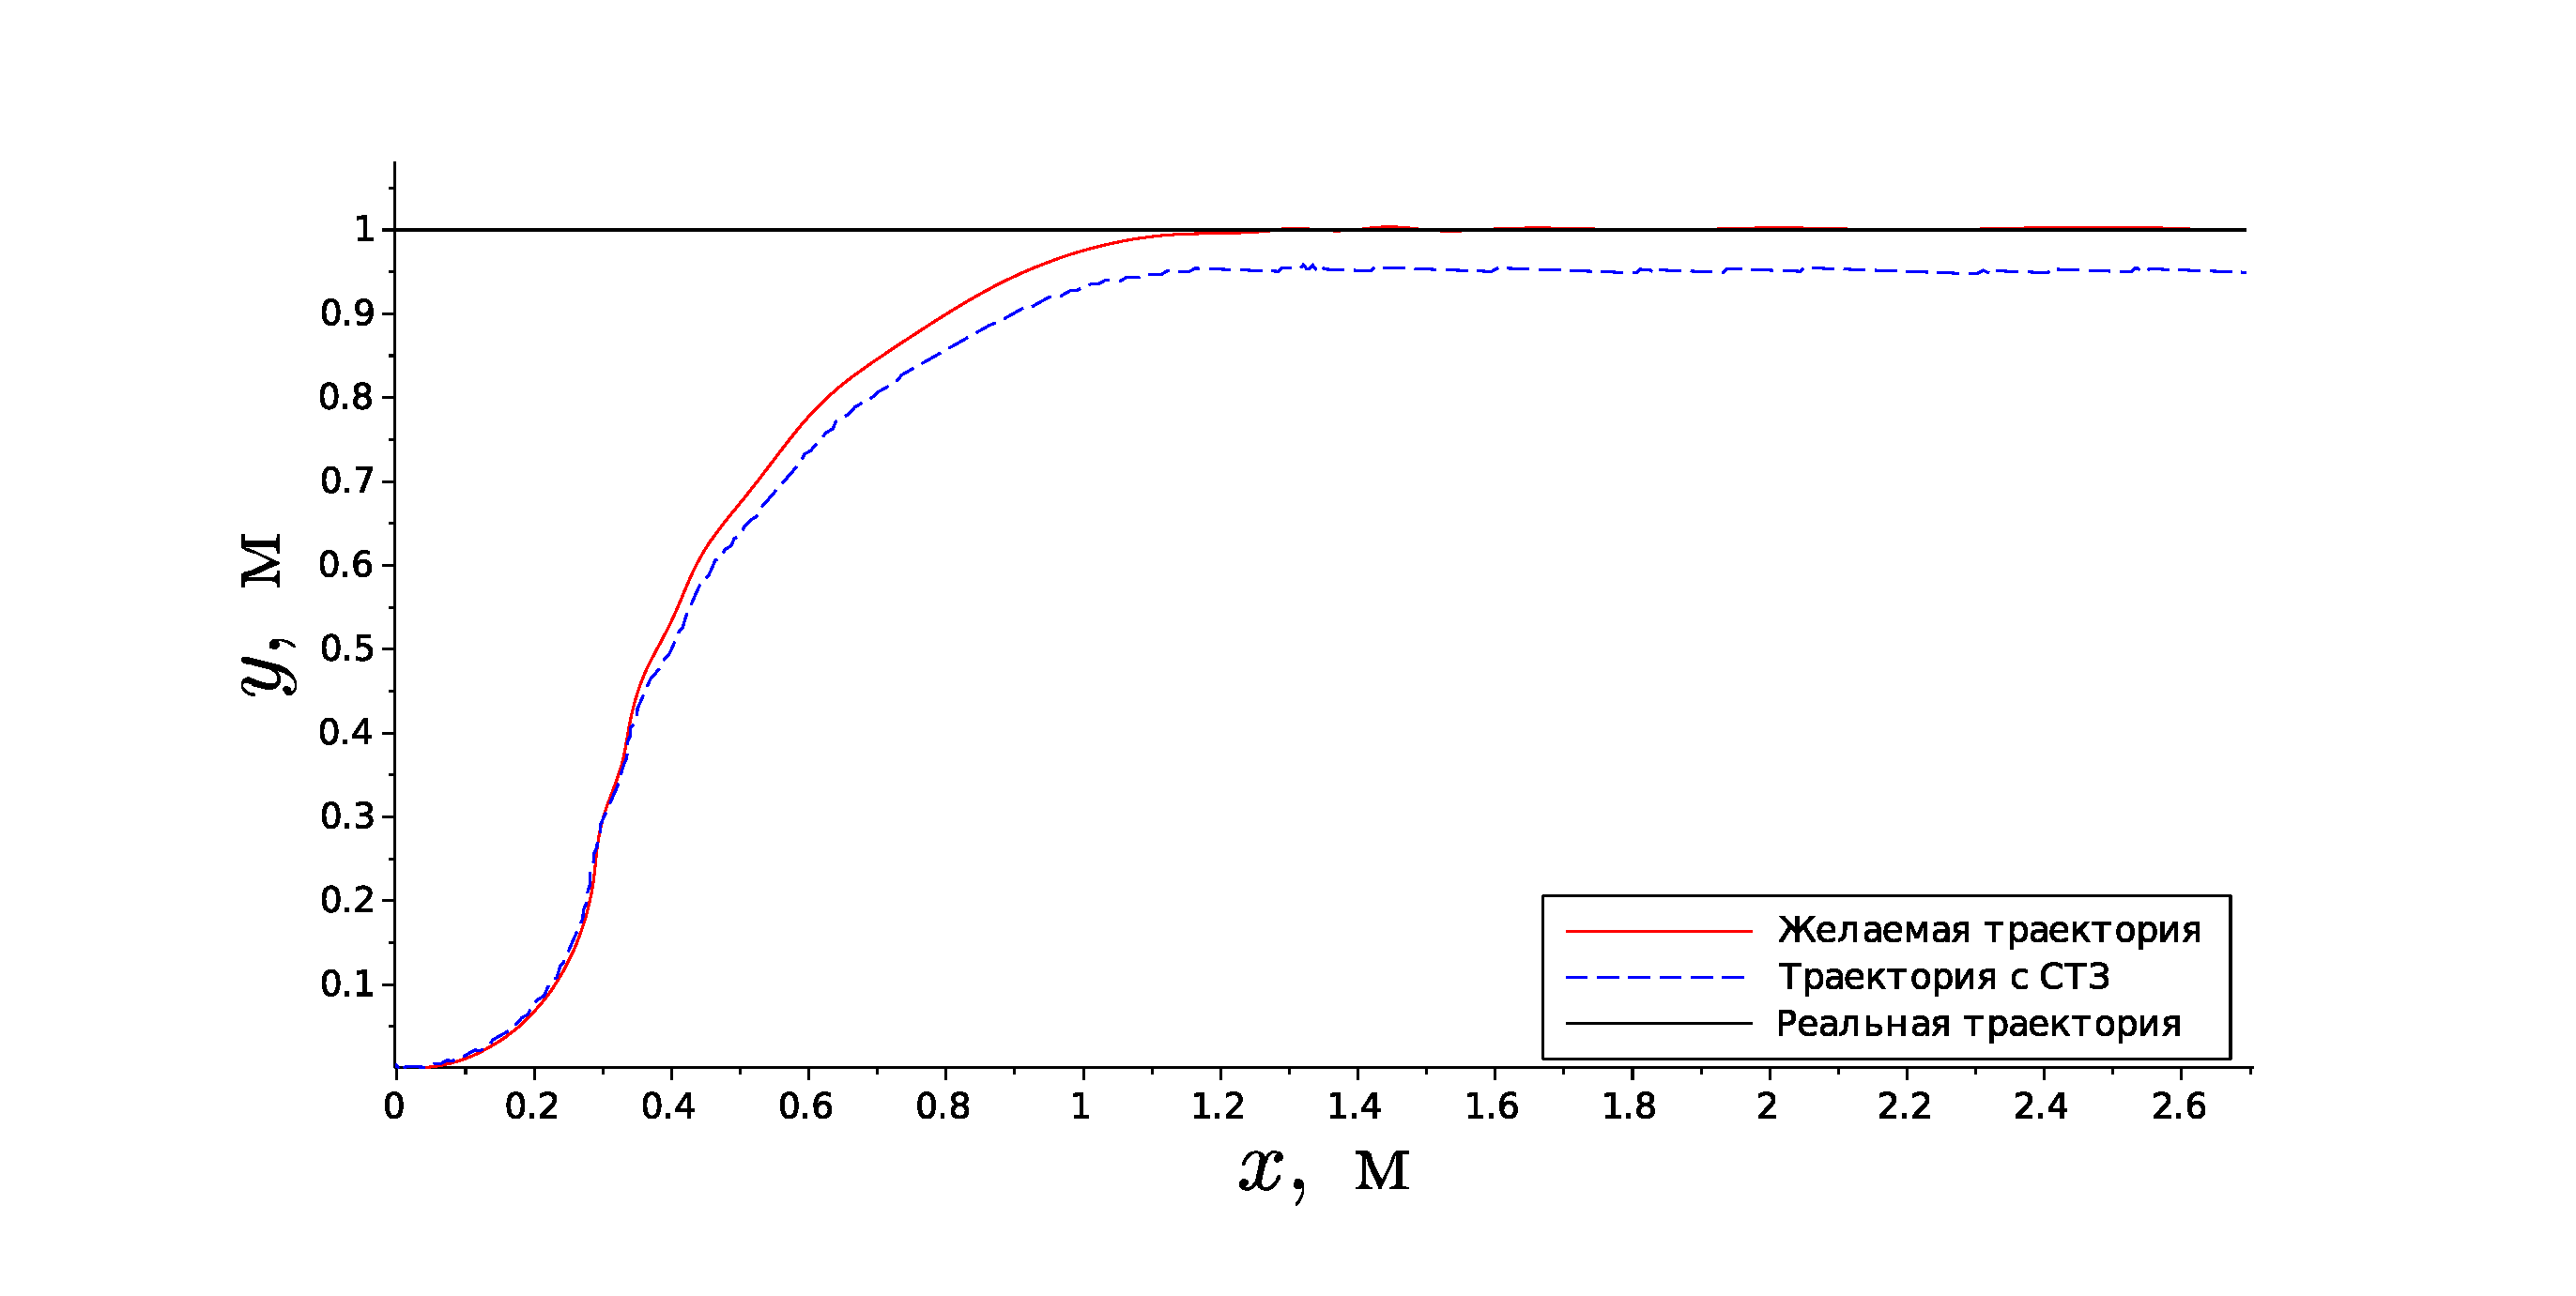
\includegraphics[width=\textwidth]{cv_trajectory.pdf}
	\caption{Траектория движения робота, полученная из СТЗ}
	\label{cv_trajectory}
\end{figure}

\begin{figure}[h]
	\centering
	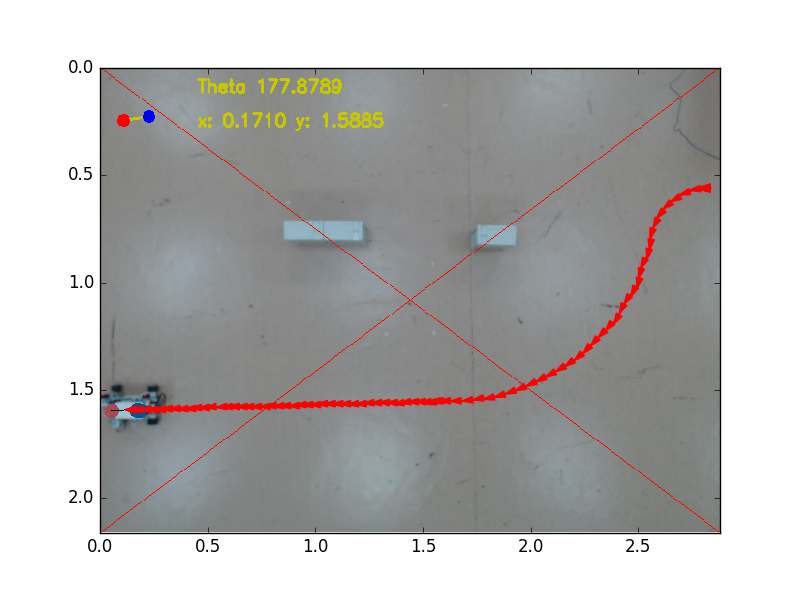
\includegraphics[width=0.9\textwidth]{cv_6.png}
	\caption{Траектория движения робота. Вид с камеры}
	\label{cv_trajectory_real}
\end{figure}

Возможным решением проблем возникших с СТЗ авторам работы видится следующие соображения:
\begin{enumerate}
	\item необходимо откалибровать камеру;
	\item закрепить камеру так, чтобы она не смещалась с течением времени (плоскость пола была строго перпендикулярна оптической оси камеры);
	\item произвести насколько это возможно более точные измерения высоты (от пола до камеры);
	\item для перевода размеров объектов в кадре из пикселей в метры использовать угол обзора камеры (сейчас используется вручную измеренные величины);
	\item повторить описанный выше эксперимент с проверкой СТЗ.
\end{enumerate}